\documentclass{article}

% 312 Font
\usepackage{charter}
% Custom lists
\usepackage{enumitem}
% Page margins & pagestyles
\usepackage{fullpage}
% Font encoding
\usepackage[T1]{fontenc}
% Colored boxes around the 'solution' environment
\usepackage{mdframed}
% Used for making FSMs
\usepackage{tikz}
\usetikzlibrary{automata}
% For color
\usepackage[dvipsnames]{xcolor}

% Defines a solution environment that creates a green box around text inside.
\mdfdefinestyle{SolutionFrame}{linecolor=green!60!black,linewidth=1pt}
\newenvironment{solution}{\begin{mdframed}[style=SolutionFrame]}{\end{mdframed}}

% Enumerate with (a),(b),(c),...
\newenvironment{enum}{\begin{enumerate}[label={(\alph*)}]}{\end{enumerate}}

% Put a dot after section titles
\renewcommand\thesection{\arabic{section}.}
\renewcommand\thesubsection{\arabic{section}.\arabic{subsection}.}

% Tikz styles & configs
\tikzset{
    ->,
    node distance=3cm,
    initial text=$ $,
}

% Images {img_size = 0.9, file_path}
\newcommand{\img}[2][0.9]{
    \begin{minipage}[t]{0.9\linewidth}
        \begin{center}
            \includegraphics[width=#1\linewidth]{#2}
        \end{center}
    \end{minipage}
}

% Hide the Date
\date{}
% Hide page numbers
\pagenumbering{gobble}

\begin{document}
    \begin{titlepage}
        \centering
        \null
        \vspace{5cm}
        {\Huge CSE 369 Lab 6\par}
        \vspace{0.5cm}
        {\Large Communicating Sequential Logic \par}
        \vfill
        {\hfill \Large Isaac Wu \par}
        {\hfill \large 2360957 \par}
        {\hfill \large \today \par}
    \end{titlepage}

\section{Top-Level Block Diagram}
    \begin{solution}
        \img{block_diagram.png} \\
        This is my Top-Level Block Diagram for the Tug-of-War module. The Tug-of-War module takes in 3 inputs, KEY0 (for Player 1), KEY3 (for Player 2), and SW9 as the Reset input. These 3 inputs go through two D flip-flops to synchronize the inputs for metastability. I then pass in the user inputs into an Edge Detector to reduce each button press to one cycle in length since our clock is very fast. Then, I pass the configured user inputs into each of the 9 light modules. These light modules have their own state and will determine whether or not their linked LED will be lit, which is output to the LEDRs outside of the ToW module. I also pass the user inputs into a Victory Display module, which controls the HEX0 display depending on if there has been a winner and if so, who won.
    \end{solution}

\newpage
\section{Edge Detector}
    \subsection{Finite State Machine}
    \begin{solution}
        Input: \{User Input, Reset\} \\
        Output: \{Edge output\}
        \begin{center}
        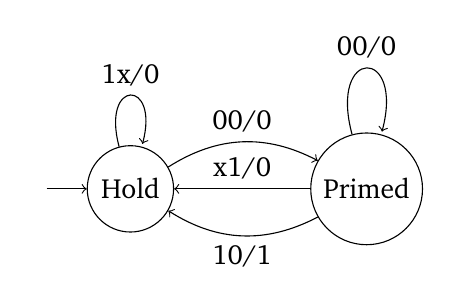
\begin{tikzpicture}
            \node[state, initial] (0) {Hold};
            \node[state, right of=0] (1) {Primed};

            \path
                (0)edge[bend left] node[above] {00/0}(1)
                (1)edge[bend left] node[below] {10/1}(0)
                (0)edge[loop above] node[above] {1x/0}(0)
                (1)edge[loop above] node[above] {00/0}(1)
                (1)edge node[above] {x1/0}(0)
             ;
        \end{tikzpicture}
        \end{center}
    \end{solution}

    \subsection{ModelSim Simulation}
    \begin{solution}
        These are the resulting waves of a simple test bench created to verify the functionality of the Edge Detector module. As seen below, when the input is active for one clock cycle, the output is also active for only one clock cycle, as expected. When the input is held for longer than one clock cycle, the edge detector output is still only active for one cycle. \\
        \img[1]{edge_waves.png}
    \end{solution}

\newpage
\section{Lights}
    \subsection{Finite State Machine}
    \begin{solution}
        Input: \{Left Input, Right Input, Left Light, Right Light, Reset\} \\
        Output: \{Light Output\} \\
        Initial Status and Reset Position is passed in as a parameter
        \begin{center}
        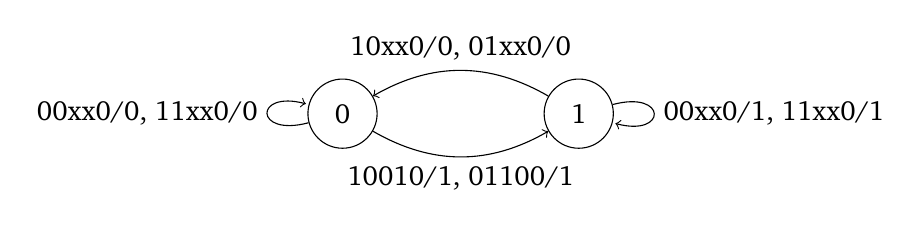
\begin{tikzpicture}
            \node[state] (0) {0};
            \node[state, right of=0] (1) {1};
            \path
                (0)edge[bend right] node[below] {10010/1, 01100/1}(1)
                (1)edge[bend right] node[above] {10xx0/0, 01xx0/0}(0)
                (0)edge[loop left] node[left] {00xx0/0, 11xx0/0}(0)
                (1)edge[loop right] node [right] {00xx0/1, 11xx0/1}(1)
            ;
        \end{tikzpicture}
        \end{center}
    \end{solution}

    \subsection{ModelSim Simulation}
    \begin{solution}
        These are the resulting waves for a test bench for the light modules. I defined two light modules, a `normal' light and a `center' light. The only difference between these two is the parameter I passed in for its initial state and reset state (0 for normal, 1 for center). I do use the same set of inputs for both lights. There are inputs that are defined as not near the lights--the normal light does not turn on and the center light turns off since the input moves the lit state away from the center. I then test various ways to turn on each light from the left and right, and the reset state. \\
        \img[1]{light_waves.png}
    \end{solution}

\newpage
\section{Victory Display}
    \subsection{Finite State Machine}
    \begin{solution}
        Input: \{Left Input, Right Input, Left-most Light, Right-most Light, Reset\} \\
        Output: \{HEX Display Output\}
        \begin{center}
        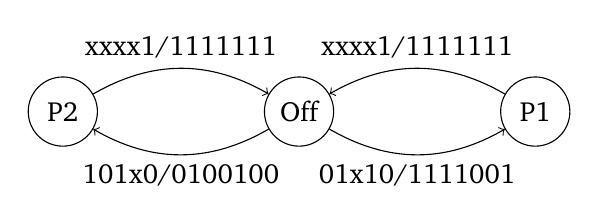
\begin{tikzpicture}
            \node[state] (O){Off};
            \node[state, left of=O] (L){P2};
            \node[state, right of=O] (R){P1};

            \path
                (O)edge[bend right] node[below]{01x10/1111001}(R)
                (R)edge[bend right] node[above]{xxxx1/1111111}(O)
                (O)edge[bend left] node[below]{101x0/0100100}(L)
                (L)edge[bend left] node[above]{xxxx1/1111111}(O)
            ;
        \end{tikzpicture}
        \end{center}
    \end{solution}

    \subsection{ModelSim Simulation}
        \begin{solution}
            This is the wave diagram for a test bench used to test the HEX output, controlled by the Victory module. After a reset input, the HEX output is defined as empty. With inputs not near the ends of the LEDs, the output doesn't change. However, if the module receives a left input, no right input, and the left-most LED is active, then the HEX display will change to show a 2 to indicate Player 2 winning. The same happens for Player 1 on the right side. Note that inputs after a win don't influence the display until a reset input is received. \\
            \img{victory_waves.png}
        \end{solution}

\newpage
\section{Top-Level ModelSim Simulation}
    \begin{solution}
        This is what a wave diagram of Player 1 winning looks like. The LED status light starts in the center and moves to the right 2 cycles after each input (due to how our input synchronization works). After the status light moves off of the final LED position, the HEX display will show a 1. Inputs after a win don't change the LED output or the HEX output. \\
        \img{player1.png} \\
        This is a wave diagram of Player 2 winning. The same thing happens, just in reverse. The LED status light starts in the center and moves to the left. After it falls off the left, the HEX display will change to display a 2. Again, any inputs after a victory will not change any displays.  \\
        \img{player2.png}
    \end{solution}

\newpage
\section{Resource Utilization}
    \begin{solution}
        \img{resources.png}
    \end{solution}

\section{Misc.}
    How many hours (estimated) it took to complete this lab in total, including reading, planning, designing, coding, debugging, and testing.
    \begin{solution}
        It took around 6 hours to complete this lab.
    \end{solution}

\end{document}